% \begin{appendix}
\section{Messdaten}
% \centering
% \begin{figure}
% \includepdf[width=0.9\textwidth, pages={1}]{Bilder/Messdaten.pdf}
% \end{figure}
% \newpage
% \begin{figure}
% \includepdf[width=0.9\textwidth, pages={2}]{Bilder/Messdaten.pdf}
% \end{figure}
%
% \end{appendix}

\begin{figure}[H]
  \centering
  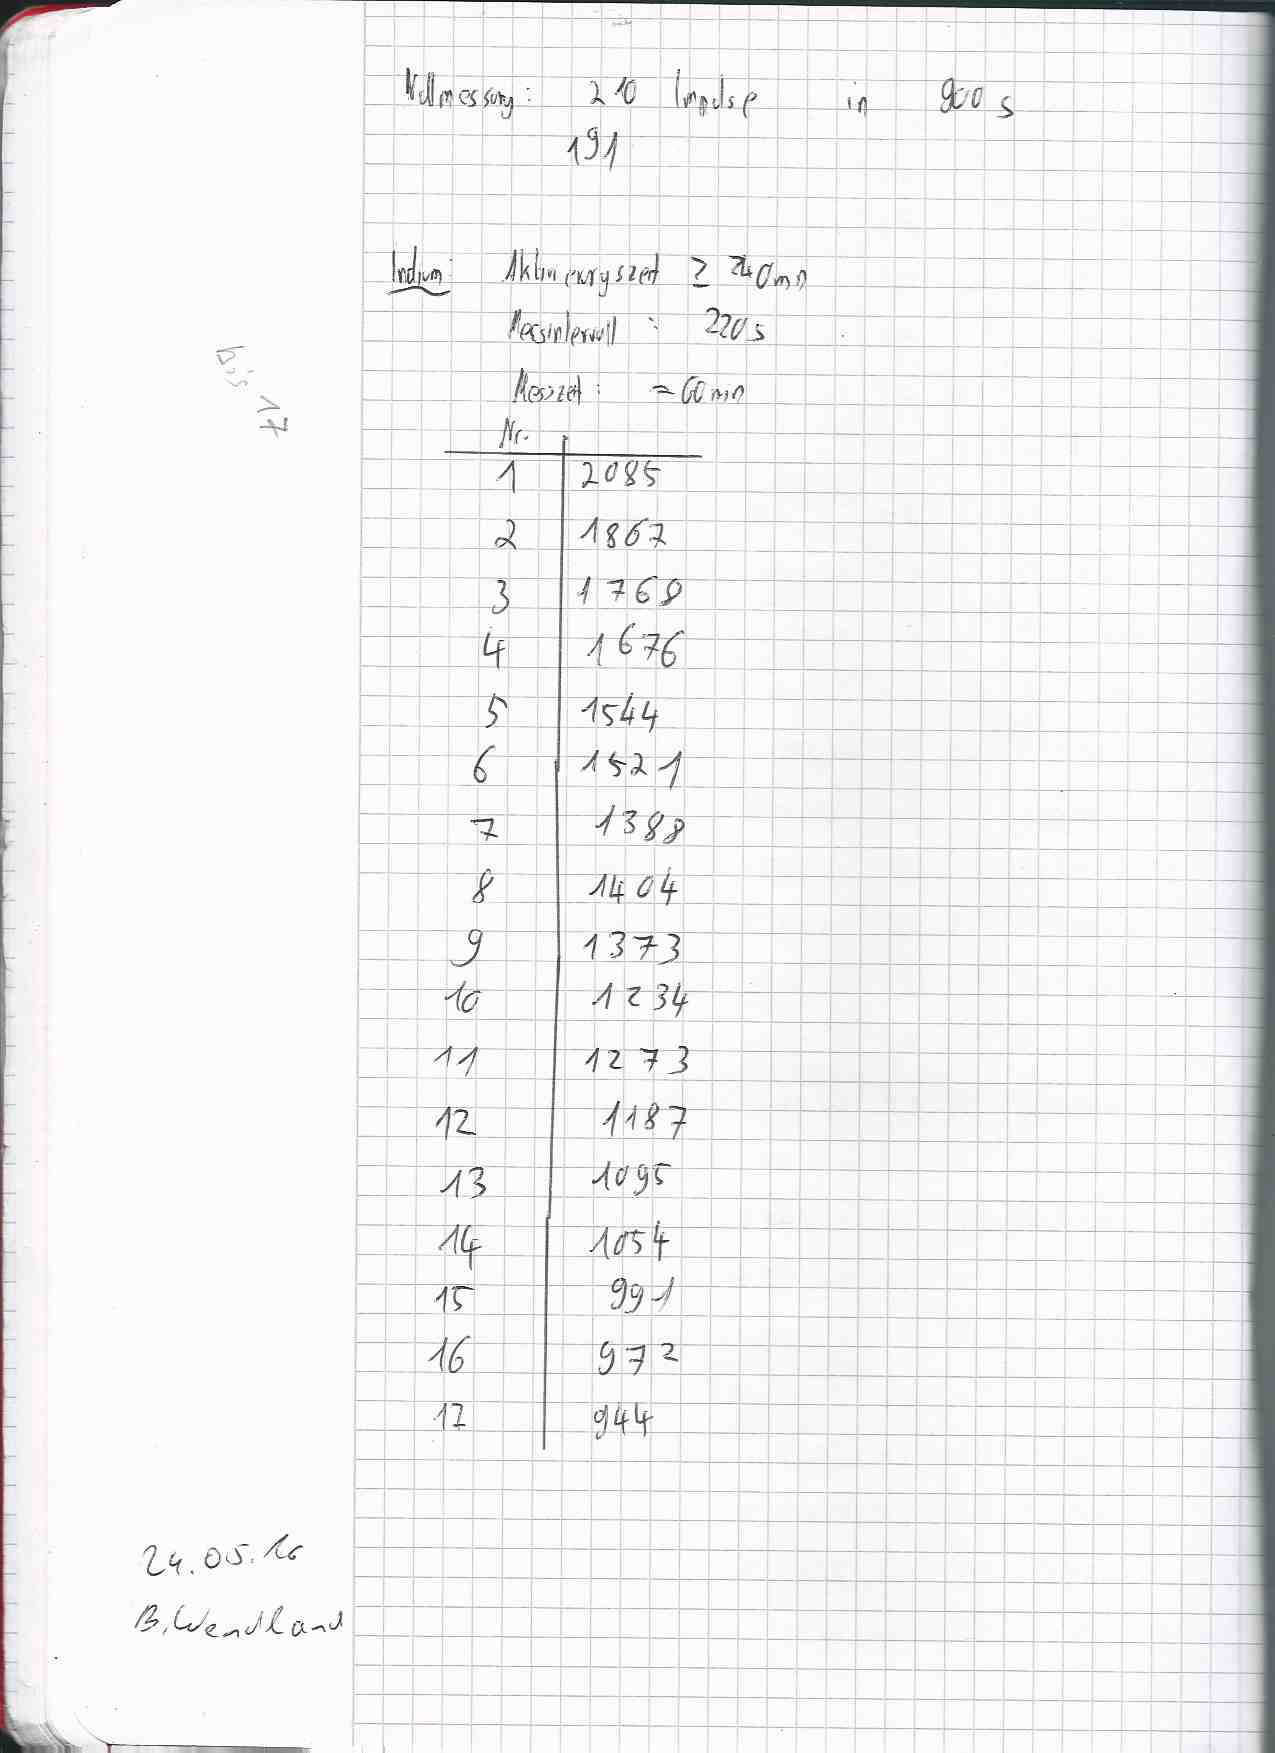
\includegraphics[page=1, height=14cm]{messdaten/scan.pdf}
  \caption{Originaldaten Teil 1.}
  \label{fig:original1}
\end{figure}

\begin{figure}[H]
  \centering
  \includegraphics[page=2, height=14cm]{messdaten/scan.pdf}
  \caption{Originaldaten Teil 2.}
  \label{fig:original2}
\end{figure}
